\documentclass[notes]{subfiles}
\begin{document}
	\addcontentsline{toc}{section}{10.4 - Areas and Lengths in Polar Coordinates}
	\refstepcounter{section}
	\fancyhead[RO,LE]{\bfseries \nameref{cs104}} 
	\fancyhead[LO,RE]{\bfseries \small \currentname}
	\fancyfoot[C]{{}}
	\fancyfoot[RO,LE]{\large \thepage}	%Footer on Right \thepage is pagenumber
	\fancyfoot[LO,RE]{\large Chapter 10.4}
	
\section*{Areas \& Lengths in Polar Coordinates}\label{cs104}
	\subsection*{Before Class}
	\subsubsection*{Area in Polar Coordinates}
		\begin{question}$ $
			\begin{enumerate}[(a)]
				\item In radian measure, what is the area of a circular wedge of radius $r$ and central angle $\theta$?
					\vs{.5}
				\item What if instead of a constant radius, we used a \emph{function} $r = f(\theta)$?  Rewrite the formula from part (a) using this new radius function.
					\vs{.5}
				\end{enumerate}
		\end{question}
		
		\begin{ex}
			This example will complete the definition of polar area.
			\begin{enumerate}[(a)]
				\item Recall the definition of the definite integral; where do the individual pieces of the definition come from?
					\vs{1}
					
				\item Consider the polar region $\mathcal{R}$ drawn below.  Label the region, and develop an approximation for a small sector, $\Delta \theta$; call the area $\Delta A_i$.
					\begin{flushleft}
					\begin{comment}
					%the code below produced the image, i just needed the graph further left than tikz was drawing it and didn't want to mess around with things
						\begin{tikzpicture}[scale = 1.25]
							\begin{polaraxis}[
								ytick = \empty,
								xtick = \empty,
								axis line style = {draw = none}
							]
								\addplot[ultra thick, domain =15:75, samples = 300] {4 - sin(3*x)};
								\addplot[thick, domain = 0:3.3, samples = 2] (15,x);
								\addplot[thick, domain = 0:4.75, samples = 2] (75,x);
							\end{polaraxis}
						\end{tikzpicture}
					\end{comment}
					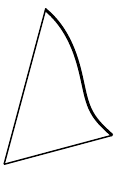
\includegraphics[scale = 1.5]{104_1.png}
					\end{flushleft}
						\newpage
						
				\item Use part (b) to develop an approximation for the area of $\mathcal{R}$, then convert the approximation to an integral.
					\vs{1}
			\end{enumerate}
		\end{ex}
		
		\begin{rmk}[Area in Polar Coordinates]
			If $r = f(\theta)$ is a continuous polar curve, then the area contained beneath $f(\theta)$ and between the angle $\theta = a$ and $\theta = b$ is given by the formula\\[20pt]
			\[A = \hspace{2in}\]
		\end{rmk}
		
		\begin{ex}
			Find the area enclosed by one loop of the four-leaved rose $r = \sin 2\theta$.
		\end{ex}
			\vs{2}
			\newpage
		
		
			
	
		
	\subsection*{Pre-Class Activities}
		\begin{ex}
			Use this space to write down any questions you might have from the videos.
		\end{ex}
			\vs{.5}
			
		\begin{ex}
			Show that the area enclosed by one loop of the rose $r = \cos 2\theta$ is exactly $\dfrac{\pi}{8}$.
		\end{ex}
			\vs{1}
			
		\begin{ex}
			Sketch the curve $r = 1-\sin \theta$, and show that its enclosed area is $\dfrac{3\pi}{2}$.
		\end{ex}
			\vs{1}
			\newpage
			
	\subsection*{In Class}
	\subsubsection*{Length in Polar Coordinates}
		\begin{rmk}[Arc Length in Polar Coordinates]
			For polar curve $r = f(\theta)$, if $f'$ is continuous on $[a,b]$, then the length of $r$ on the interval $a\leq \theta \leq b$ is given by\\[10pt]
				\[L = \hspace{2.5in}\]
		\end{rmk}
		\begin{pf}
		
		\end{pf}
			\vspace{2.5in}
			
		\begin{ex}
			Find the exact length of the curve $r = 2\cos\theta$ on the interval $0\leq \theta \leq \pi$.
		\end{ex}
			\vs{1}
			\newpage
			
	\subsubsection*{Examples}
		\begin{ex}
			Find the area of the region inside the circle $r = 3\cos\theta$ and outside the cardioid $r = 1+ \cos\theta$.
		\end{ex}
			\vs{1}
			
		\begin{ex}
			Find all points of intersection for the curves $r = \dfrac{1}{2}$ and $r =\sin 2\theta$.
		\end{ex}
			\vs{1}
			\newpage
			
		\begin{ex}
			Find the area of the region enclosed by one loop of the curve $r^2 = 4\cos 2\theta$.
		\end{ex}
			\vs{1}
		
		\begin{ex}
			Find the area of the region that lies inside $r = 1-\sin\theta$, but outside of the circle $r = 1$.
		\end{ex}
			\vs{1}
			
		\begin{ex}
			Find the area of the region inside $r = 1+\cos\theta$, and outside $r = 2-\cos\theta$.
		\end{ex}
			\vs{1}
			\newpage
			
		\begin{ex}
			Find all points of intersection for the curves $r = \sin\theta$ and $r = 1-\sin\theta$.
		\end{ex}
			\vs{1}
			
		\begin{ex}
			Find the exact length of the polar curve $r = 5^\theta$, for $0\leq \theta \leq 2\pi$.
		\end{ex}
			\vs{1}
			
		\begin{ex}
			Find the area of the region that lies between $r = 1+\cos\theta$ and $r = 1-\cos\theta$.
		\end{ex}
			\vs{1}
			\newpage
			
	\subsection*{After Class Activities}
		\begin{ex}
			Find the area enclosed by one loop of the curve $r = 4\cos 3\theta$.
		\end{ex}
			\vs{1}
			
		\begin{ex}
			Find the area between the curves $r = 3 +2\cos\theta$ and $r = 3 +2\sin\theta$.
		\end{ex}
			\vs{1}
			\newpage
			
		\begin{ex}
			Find all points of intersection of the curves $r = 2\sin2\theta$ and $r = 1$.
		\end{ex}
			\vs{1}
			
		\begin{ex}
			Find the exact length of the spiral $r = \theta^2$ on the interval $0\leq\theta\leq \sqrt{5}$.
		\end{ex}
			\vs{1}
\clearpage
\end{document}